% !TeX root = document.tex
% !TeX encoding = UTF-8 Unicode

\chapter{Simulação do Modelo}%
\label{chapter:model-simulation}

Esse módulo permite a simulação de um modelo. Na
Figura~\ref{fig:model-simulation} pode-se ver as opções de configuração da
simulação. A simulação suporta modelos contínuos e discretos, em espaço de
estados e função de transferência.

\begin{figure}[ht!]
    \centering
    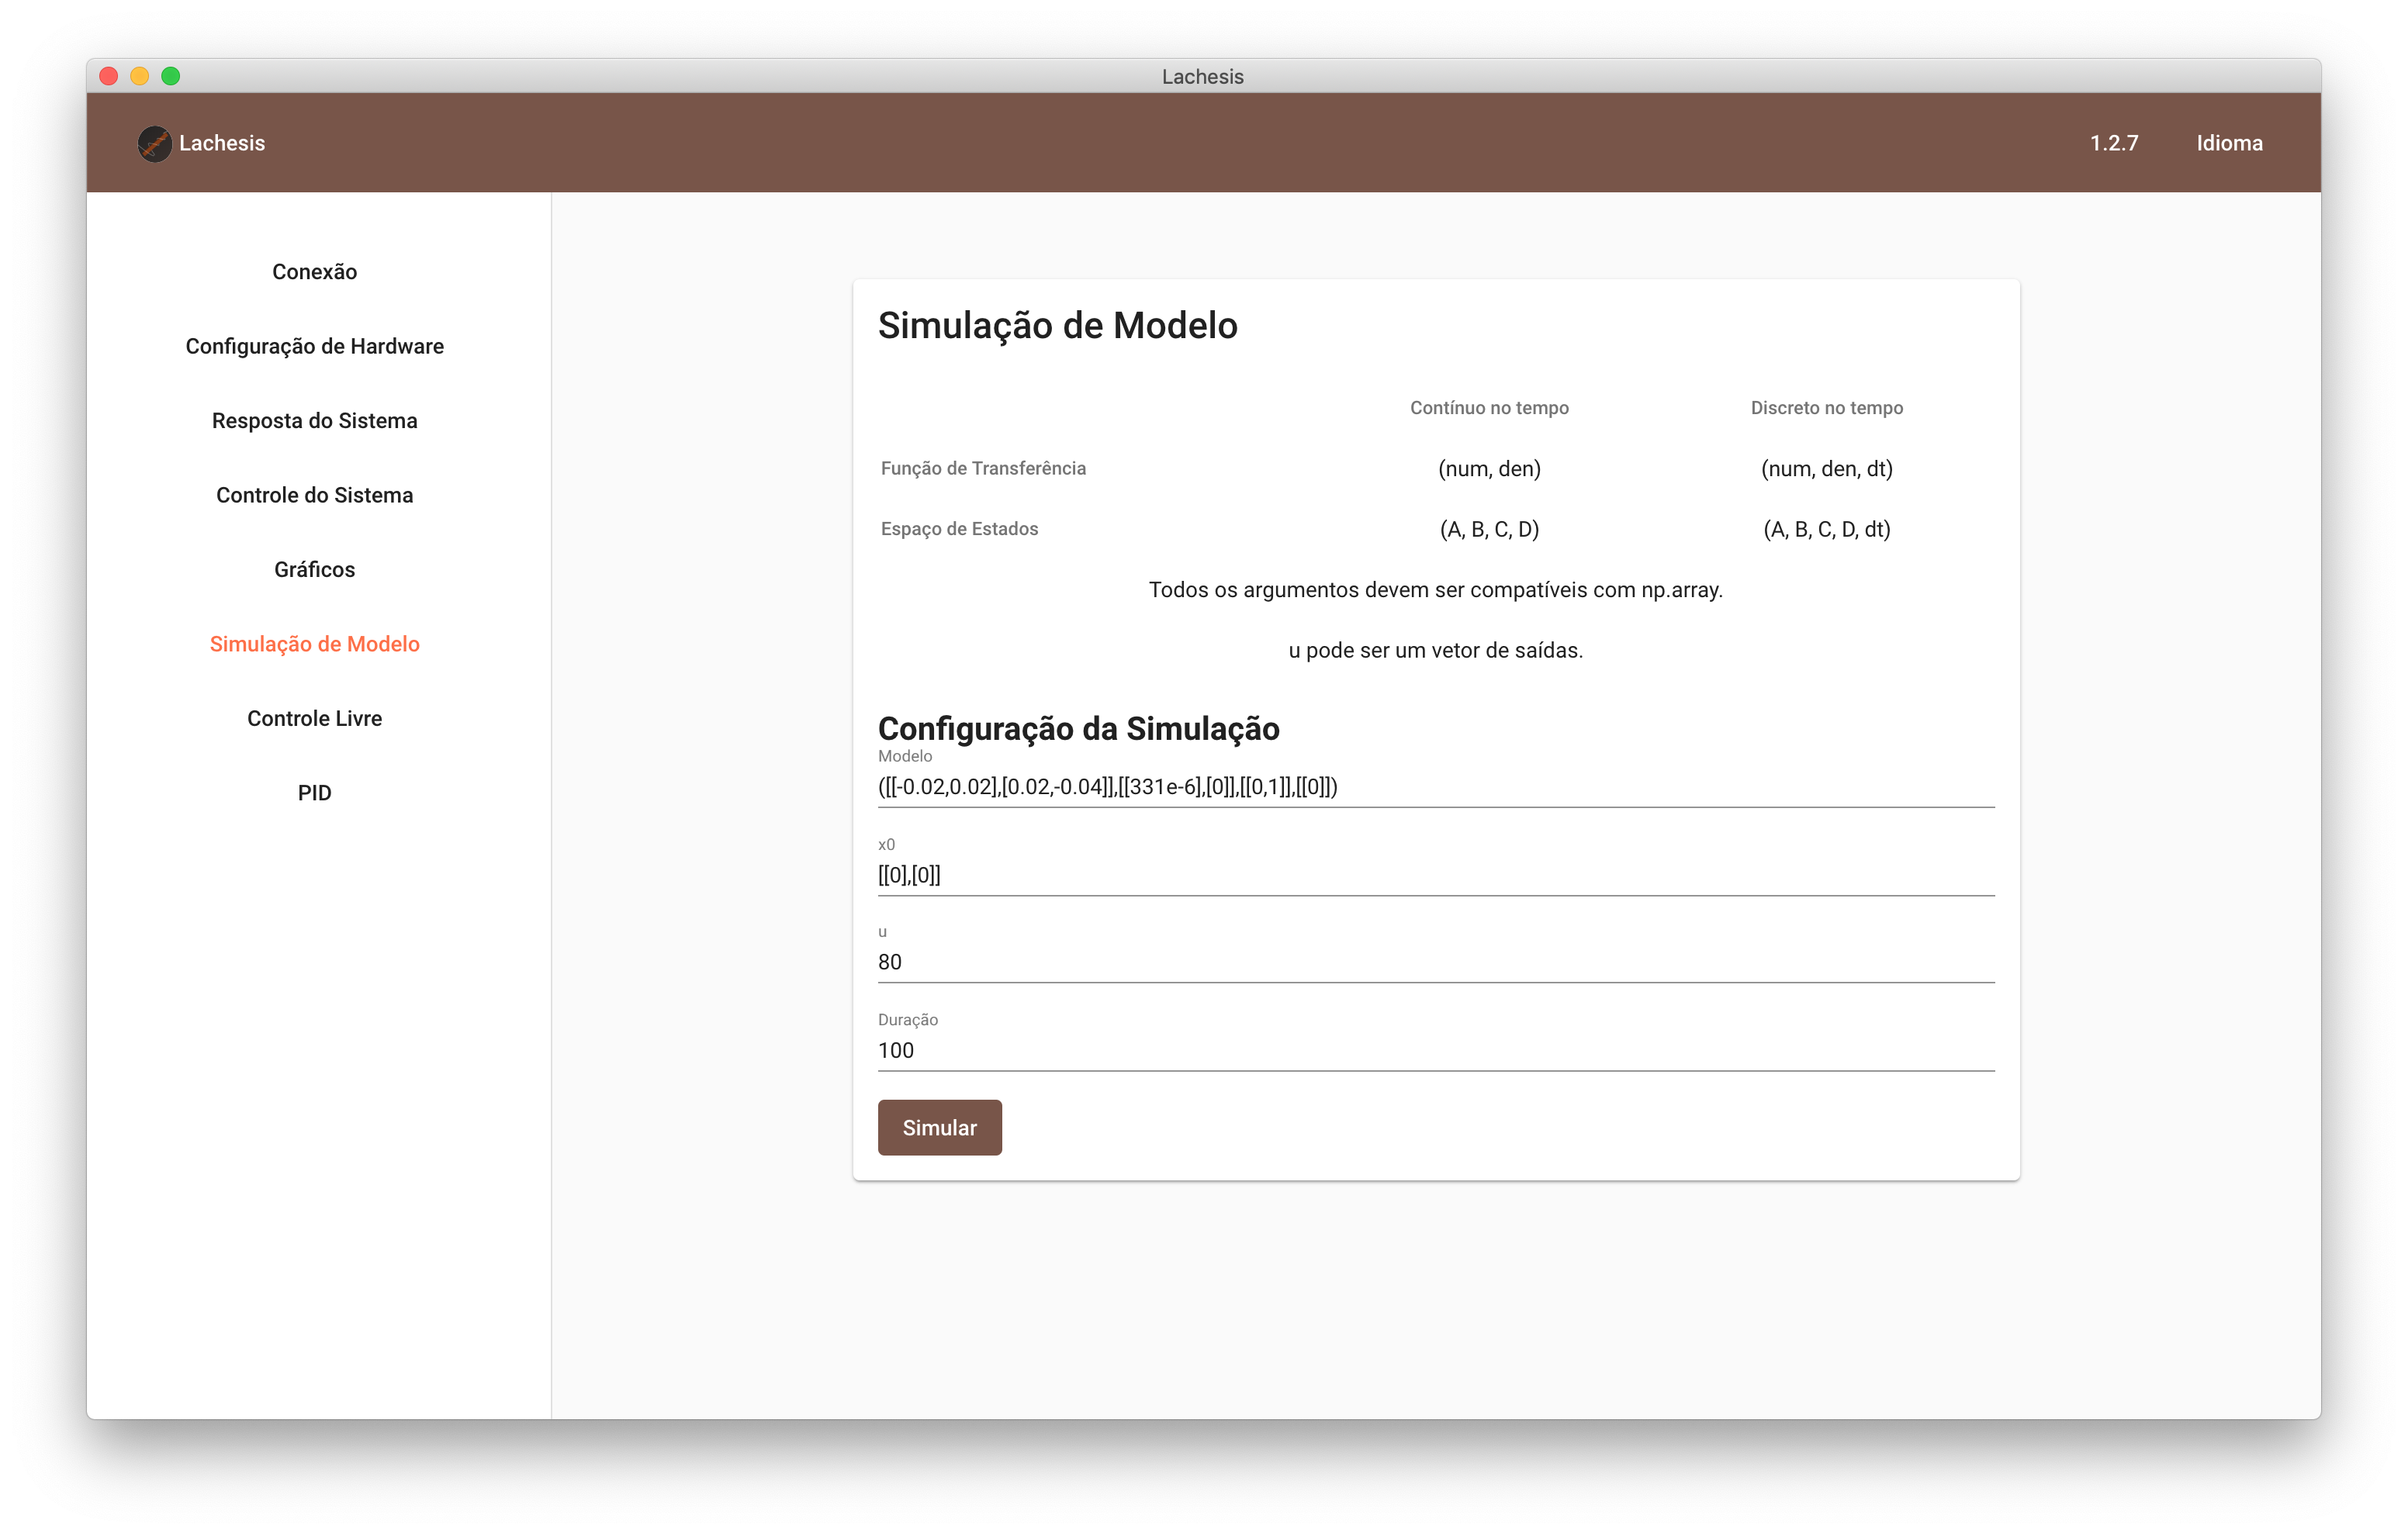
\includegraphics[width=0.9\textwidth]{imgs/model-simulation}
    \caption[Módulo Simulação de Modelo]{Módulo Simulação de Modelo}%
    \label{fig:model-simulation}
\end{figure}

Caso o modelo não esteja em espaço de estados discreto, ele será convertido para
tal. No caso de modelos contínuos, o tempo de amostragem é calculado como:

\mintinline{python}{dt = max(0.1, float('%.1f' % (max(abs(np.real(vals))) / 5)))}

em que \textit{vals} são os polos do sistema.

Caso o sinal de controle \textit{U} seja informado como um número, ele será
aplicado de forma constante pela duração da simulação. Caso seja um vetor, cada
item será aplicado por uma amostragem, e o valor do campo \textit{Duração} será
ignorado.

Assim, considerando um sistema discreto com \(\delta{}t=5\) segundos, podemos
definir um sinal de controle em rampa de 0 a 100 e retornando a zero como:

\mintinline{python}{[*range(0,100,5),*range(100,0,-5)]}.

Tal sinal de controle aplica uma variação de 5 a cada amostragem, e tem duração
de \mintinline{python}{len([*range(0,100,5),*range(100,0,-5)]) * dt}, no caso,
200 segundos.

Os campos \textit{Modelo}, \textit{x0} e \textit{U} aceitam código
\textit{Python} como entrada, como pode ser visto exemplo anterior. Como a
simulação é sempre feita em espaço de estados discreto, é sempre necessário
informar um \textit{x0} adequado.

O resultado da simulação é salva como um teste, e pode ser vista também no
módulo \textit{Gráficos}, onde é possível exportar os dados.
